\subsection{Resultados Experimentais}
\subsubsection{Relação Resistência/Tensão}
Maecenas eu volutpat turpis, in blandit nunc. Aliquam porttitor tortor eu diam mollis, et facilisis eros porttitor. Aenean purus ligula, molestie nec neque vestibulum, sagittis faucibus lectus. 

\begin{figure}[!htb]
    \centering
    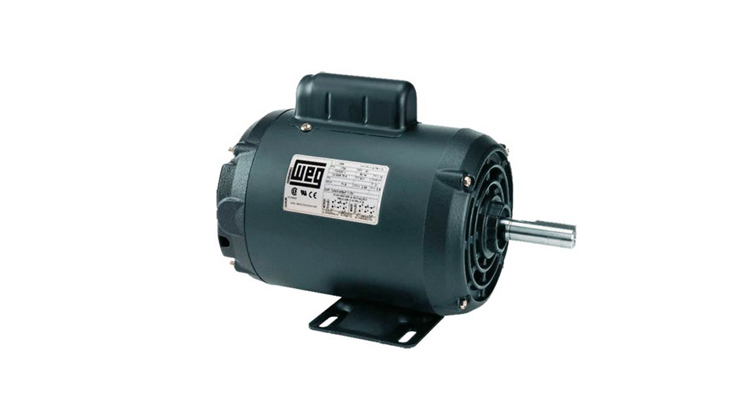
\includegraphics[scale=0.1]{motor_mono.jpg}
    \caption{Motor Monofásico}
    \label{fig:motor}
\end{figure}

Nulla sit amet lectus et sapien pretium eleifend. Nam pharetra, urna et porttitor auctor, ipsum sapien rutrum ligula, id porttitor sem lacus nec nulla. Donec imperdiet iaculis urna ut dapibus. Maecenas pulvinar semper ipsum sagittis fermentum. Fusce bibendum vestibulum volutpat. Vestibulum ante ipsum primis in faucibus orci luctus et ultrices posuere cubilia curae; Donec ac sem gravida, egestas lacus ac, molestie tortor. Lorem ipsum dolor sit amet, consectetur adipiscing elit. Sed gravida semper viverra. Vestibulum venenatis dolor eu augue tincidunt, a egestas sapien eleifend. Aliquam erat volutpat. 

\begin{table}[!htb]
    \centering
    \begin{tabular}{c|c}
    \hline
    Resistência & Tensão \\ \hline
    $20 \Omega$ & 2V \\
    $10 \Omega$ & 4V \\
    $0.5\Omega$ & 100V \\ \hline
    \end{tabular}
    \caption{Relação resistência/Tensão}
    \label{tab:relação res/ten}
\end{table}

\subsection{Relação Corrente/Luminosidade}
Maecenas eu volutpat turpis, in blandit nunc. Aliquam porttitor tortor eu diam mollis, et facilisis eros porttitor. Aenean purus ligula, molestie nec neque vestibulum, sagittis faucibus lectus. Cras sit amet ante sed diam ornare ultrices vitae ac justo. Nunc nec imperdiet est, eget bibendum nisl. Sed consectetur risus viverra auctor aliquet. Etiam quis rhoncus ante. 
\begin{table}[!htb]
\centering
\begin{tabular}{|c|c|}
\hline
Corrente & Luminosidade \\ \hline
2A       & 1lm          \\ \hline
3A       & 3lm          \\ \hline
4A       & 5lm          \\ \hline
5A       & 7lm          \\ \hline
6A       & 10lm         \\ \hline
\end{tabular}
\caption{Relação Corrente Luminosidade}
\label{tab:Relação corrente lum}
\end{table}

\subsubsection{Nota dos Materiais}
Maecenas eu volutpat turpis, in blandit nunc. Aliquam porttitor tortor eu diam mollis, et facilisis eros porttitor. Aenean purus ligula, molestie nec neque vestibulum, sagittis faucibus lectus. Cras sit amet ante sed diam ornare ultrices vitae ac justo. Nunc nec imperdiet est, eget bibendum nisl. Sed consectetur risus viverra auctor aliquet. Etiam quis rhoncus ante. 

\begin{table}[!htb]
\centering
\caption{Nota dos Materiais}
\begin{tabular}{lllll}
\hline
\multicolumn{1}{|l|}{} & \multicolumn{1}{l|}{Metal} & \multicolumn{1}{l|}{Polímero} & \multicolumn{1}{l|}{Cerâmica} & \multicolumn{1}{l|}{Semicondutor} \\ \hline
Tensão                 & 10                         & 0                             & 0                             & 7                                 \\
Corrente               & 10                         & 0                             & 0                             & 9                                 \\
Luminosidade           & 10                         & 8                             & 2                             & 0                                
\end{tabular}
\label{tab:nota dos materiais}
\end{table}

\subsection{Resultados Teóricos}
Nulla sit amet lectus et sapien pretium eleifend. Nam pharetra, urna et porttitor auctor, ipsum sapien rutrum ligula, id porttitor sem lacus nec nulla. Donec imperdiet iaculis urna ut dapibus. Maecenas pulvinar semper ipsum sagittis fermentum. Fusce bibendum vestibulum volutpat. Vestibulum ante ipsum primis in faucibus orci luctus et ultrices posuere cubilia curae; Donec ac sem gravida, egestas lacus ac, molestie tortor. Lorem ipsum dolor sit amet, consectetur adipiscing elit. Sed gravida semper viverra. Vestibulum venenatis dolor eu augue tincidunt, a egestas sapien eleifend. Aliquam erat volutpat. 

$$
    \zeta = \left( \begin{array}{cc}
        2\tau & 7\phi-\frac{5}{12} \\
        3 \psi & \frac{\pi}{8}
    \end{array} \right)
    
$$